\section{Multiplication in Three Operands}
The very first component of the ALU should be the circuit that calculates the result of
\textbf{\(A^2\ast B\)}.
Hence the multiplication of two 8-bit operands circuits should be designed first,
then the circuit for multiplying the product of the square A with the B should be designed later.

In general, the multiplication of two 8 bits operands in the shift-and-add algorithm or the radix-2 booth
algorithm requires 8 steps of calculating eight partial products and then adding them together.
By using the modified booth algorithm which is also known as radix-4 booth algorithm,
the number of the partial products can be reduced to 2/n where n is the bit length of the operand.

Not only because it’s faster, but also because it saves more area compared with the previous two algorithms.
Hence the project chooses to implement the radix-4 booth algorithm as the multiplication component of the ALU.

There is an extra partial product the circuit should consider since the booth algorithm is designed for the sighed number.
In this case, the implemented algorithm requires 2/n + 1 partial product for the unsigned number to reach the final answer.
This will be discussed in the following sections.

\subsection{Radix-4 Booth Algorithm Logic in Details}

Booth algorithm calculates the partial product by examining the “Code Table” on the second operand, the multiplier.
The table requires certain blocks of bits from the right side to the left side of the multiplier, and for each block,
the table provides the partial product respectively. Radix-2 requires 2 bits while radix-4 requires 3 bits.
This is how the radix-4 algorithm reduces the partial products to a half.
In this manner, the overlaps will occur in the partial products,
hence the algorithm will do subtraction according to the “Code Table”.

\subsubsection{Example in Signed Number Multiplication}

When the algorithm is used for calculating two 8-bit signed number \textit{0b01010110} which is 86 in decimal,
and \textit{0b00100011} which is 35 in decimal, the multiplier will be decoded as \figref{fig:booth_code_1} is shown.
Then all partial products can be derived from the code blocks and the “Code Table”
which is presented in \tbref{tb:code_table}.

% do not use figure* here otherwise the picture willl postpone after the references list 
\begin{figure}[!ht]
	\centering
	\caption{The Decoded Code Blocks of the Signed Multiplier}
	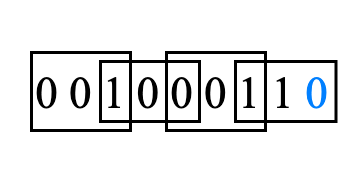
\includegraphics[width=2.7in]{../img/booth_code_1.png}
	\figurenote{The blue bit is an extra bit which is added on the right of the LSB of the multiplier for completing the first code block.}
	\label{fig:booth_code_1}
\end{figure}

\begin{table}[!ht]
	\renewcommand{\arraystretch}{1.3}
	\caption{Code Table of Radix-4 Booth Algorithm}
	\centering
	\begin{tabular}{ >{\centering\arraybackslash}p{3cm} >{\centering\arraybackslash}p{7cm} }
		\hline
		\bfseries Code Blocks & \bfseries Partial Product \\
		\hline
		000/111               & 0                         \\
		001/010               & \(1\ast multiplicand \)   \\
		011                   & \(2\ast multiplicand \)   \\
		100                   & \(-2\ast multiplicand \)  \\
		101/110               & \(-1\ast multiplicand \)  \\
		\hline
	\end{tabular}
	\label{tb:code_table}
\end{table}

The algorithm takes four blocks of code from the right to the left and retrieves the corresponding product by shifting two bits more than the previous product.
Then perform the addition. The process of the algorithm is described in \figref{fig:r4b_process_1}.

\begin{figure}[!ht]
	\centering
	\caption{Process of the Algorithm for Signed Number}
	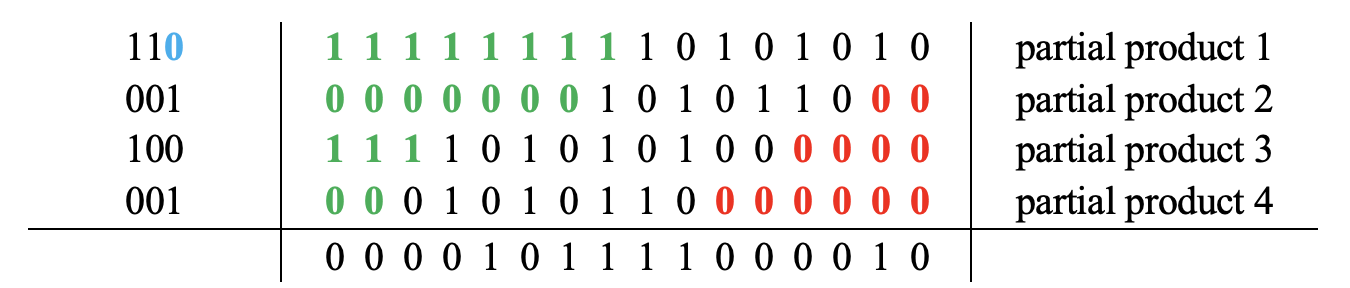
\includegraphics[width=5.7in]{../img/r4b_process_1.png}
	\figurenote{Bits in green color represent the product is extended to 16 bits. Bits in red color represent the shifted 2 bits leftward.}
	\label{fig:r4b_process_1}
\end{figure}

After the performance, the result \textit{0b0000101111000010} is 3010 in decimal which is the product of 86 and 35.
As can be observed at the table, subtraction can be done by adding the negation of the number which is represented
by 2’s complement.

\subsubsection{Example in Unsigned Number Multiplication}

Applying the algorithm to unsigned operands is a little bit different.
Because the MSB of the operand is treated as a valid number rather than the sign,
the operands should extend to 9-bit by adding a “0” to the MSB. Hence an extra partial product will be added to the product.
For instance, multiplicand \textit{0b010010101} which is 149 in decimal and multiplier \textit{0b011001100}
which is 204 in decimal can be operated in the process as \figref{fig:r4b_process_2} and \figref{fig:r4b_process_2} are shown.

\begin{figure}[!ht]
	\centering
	\caption{The Decoded Code Blocks of the Unsigned Multiplier}
	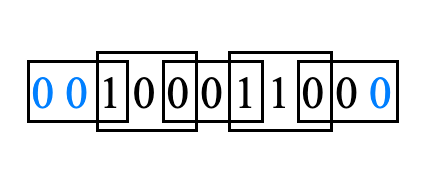
\includegraphics[width=3in]{../img/booth_code_2.png}
	\figurenote{Two “0” are added to the MSB to complete the last code block. The second zero represent the sign bit of the operand which in this case will always be positive number.}
	\label{fig:booth_code_2}
\end{figure}

\begin{figure}[!ht]
	\centering
	\caption{Process of the Slgorithm for Unisgned Number}
	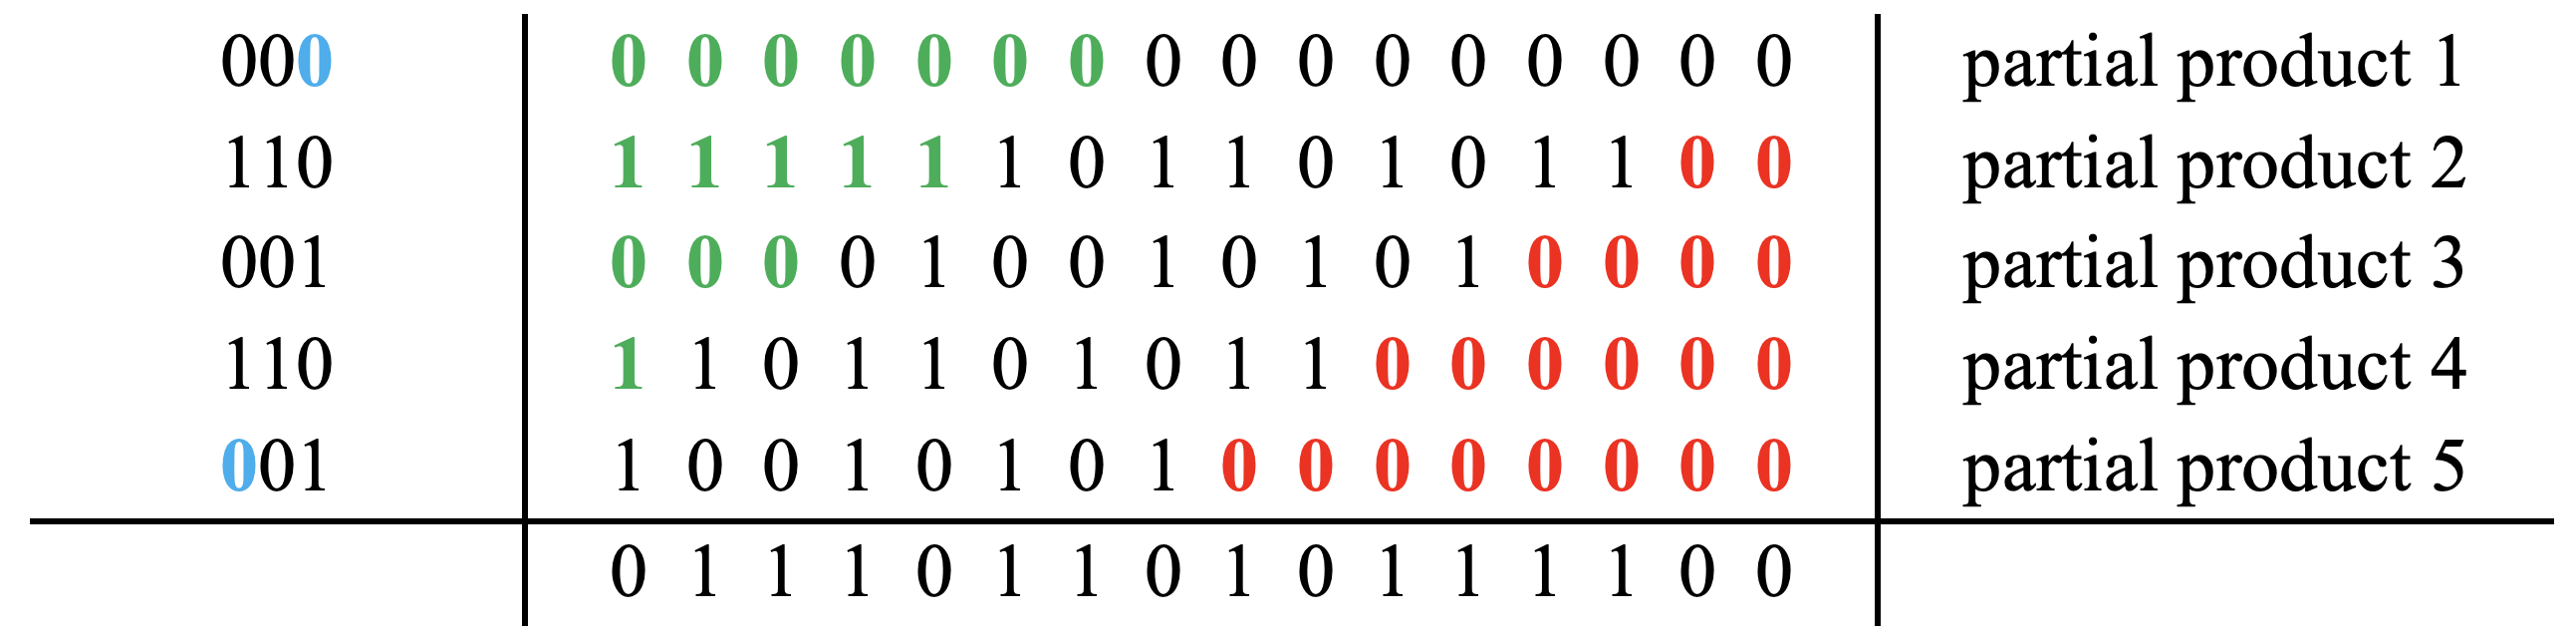
\includegraphics[width=5.7in]{../img/r4b_process_2.png}
	\figurenote{Bits in green color represent the product is extended to 16 bits. Bits in red color represent the shifted 2 bits leftward.}
	\label{fig:r4b_process_2}
\end{figure}

\subsection{8-bit Radix-4 Booth Multiplier Circuit Implementation}
\subsubsection{Overall Circuit Design and RTL Description}

As the previous discussion, the booth multiplier component should contain the following blocks: 1.
A 9-bit complement generator for the negation of the multiplicand;
2. Five booth stage units for 5 partial products;
3. Four 16-bit adders to sum up the partial products.
\figref{fig:overview_booth_rtl} presents the synthesized RTL diagram of the multiplier circuit.

\begin{figure}[!ht]
	\centering
	\caption{Synthesized RTL Diagram of 8-bit Radix-4 Booth Multiplier}
	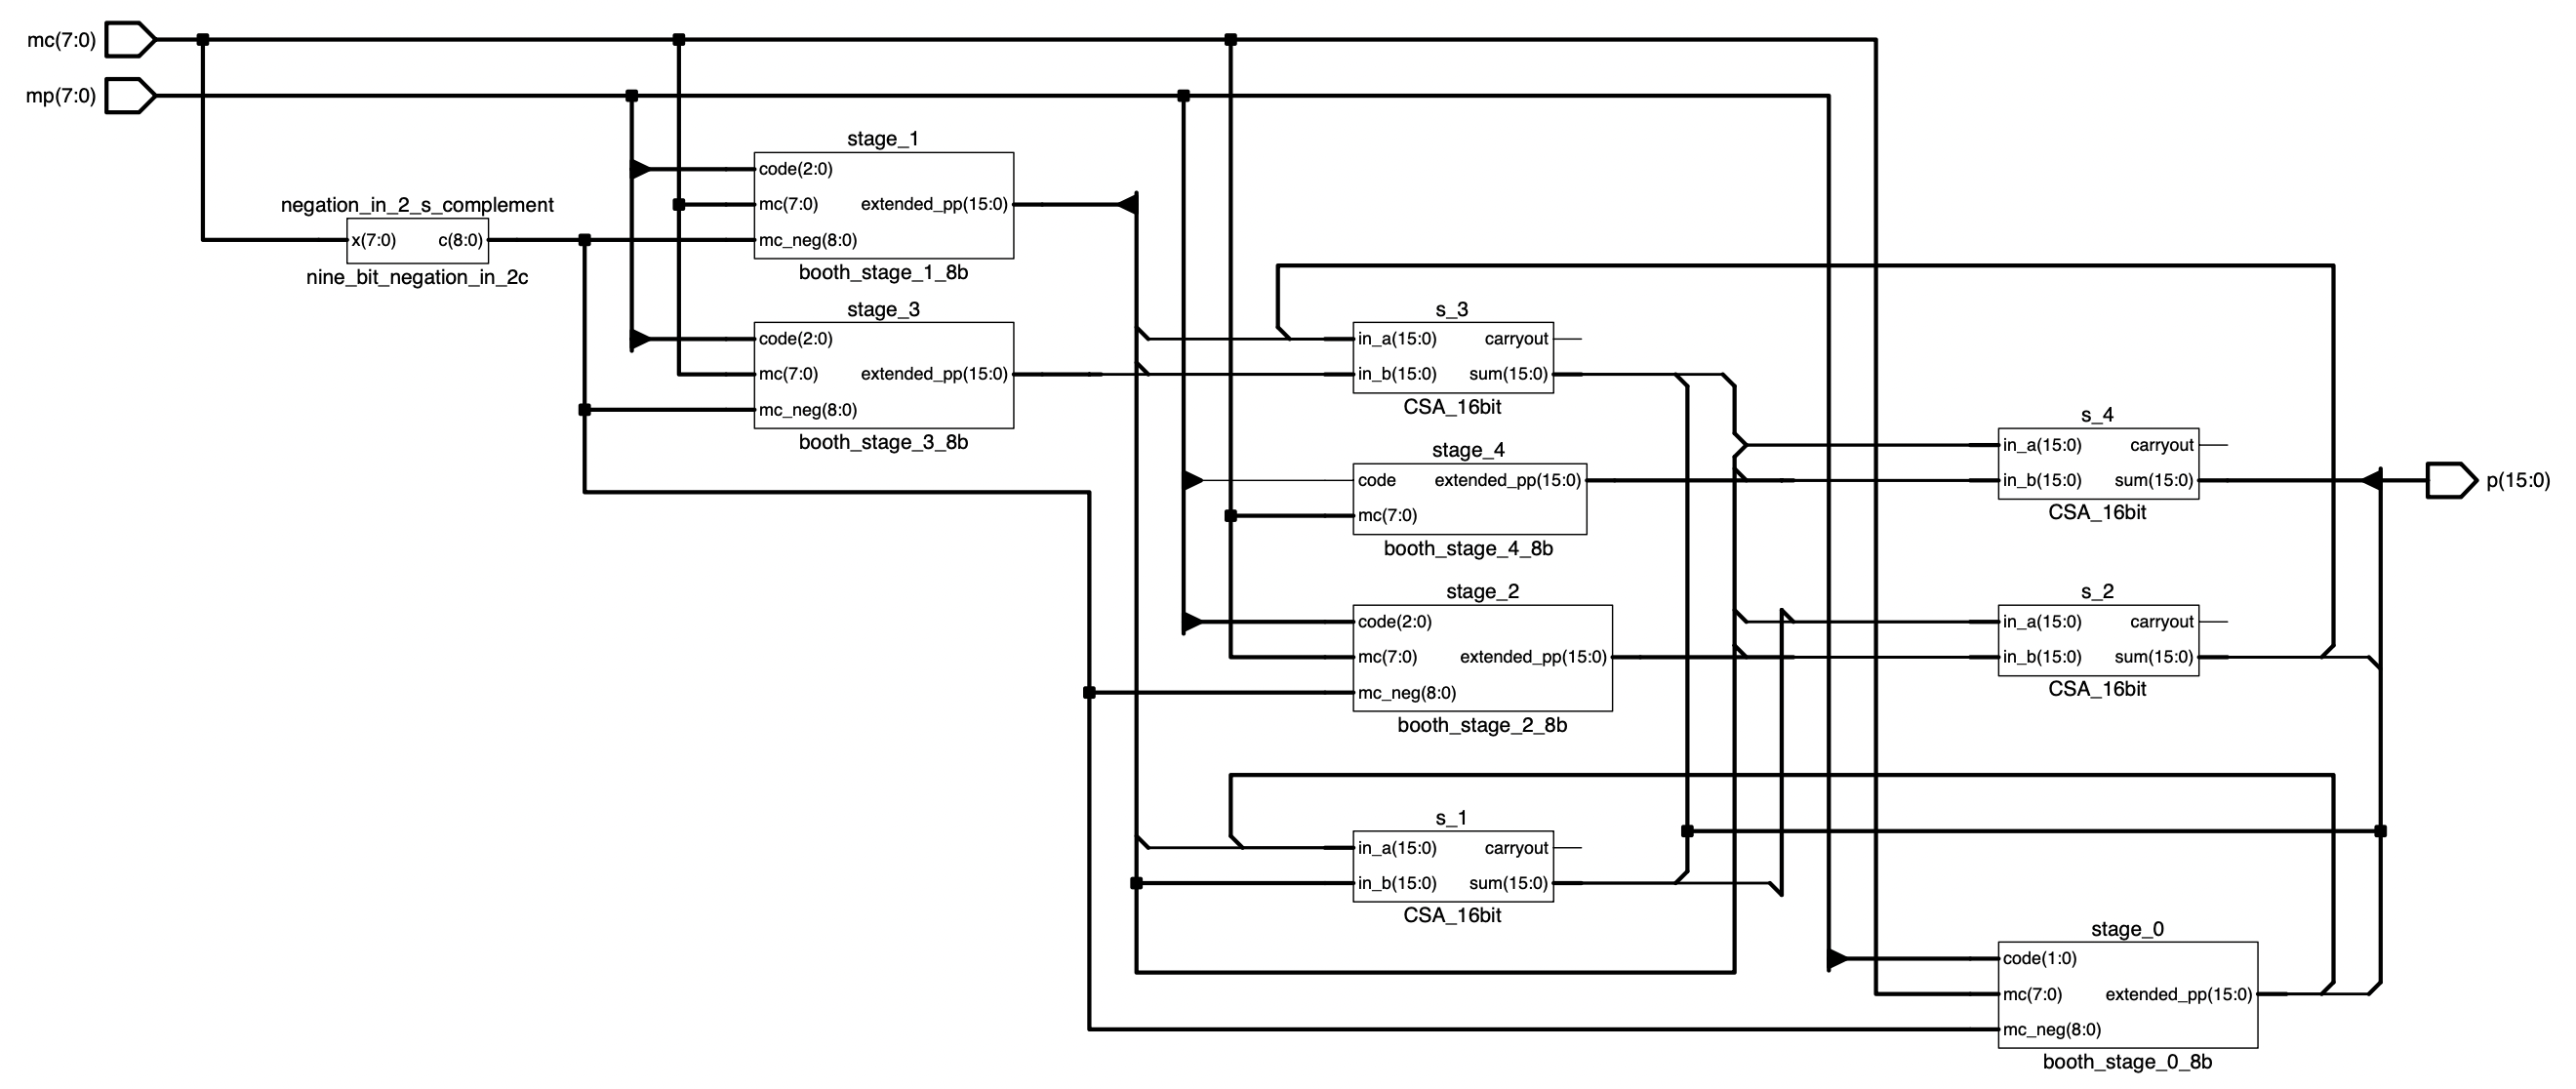
\includegraphics[width=\textwidth]{../img/overview_booth_rtl.png}
	\label{fig:overview_booth_rtl}
\end{figure}

The circuit will first calculate a 9-bit negation of operand multiplicand in 2's complement.
Then pass through all five booth stage blocks to get five 16-bit partial products.
And finally sums those partial products up.

\subsubsection{Blocks Design}

This section will discuss the design of the complement generator and five of the booth stages,
the 16-bit CSA will be discussed in Section “Carry Select Adder”.

\paragraph{The 9-bit Complement Generator for the Negation of the Multiplier}
Since the circuit uses negation addition to represent the subtraction, a complement generator should be introduced.
The RTL diagram of the generator is shown in \figref{fig:complementor_rtl}.
The logic of the generator that uses a 2-to-1 mux is straightforward as \expref{exp:complementor_exp} described.
The simulation result is shown in \figref{fig:complementor_sim}.

\begin{equation}
	c =
	\begin{cases}
		concat(0, x),                 & \text{if } x = 00000000 \\
		concat(1,\ (not\ \ x))\ +\ 1, & \text{otherwise}
	\end{cases}
	\label{exp:complementor_exp}
\end{equation}

\begin{figure}[!ht]
	\centering
	\caption{Synthesized RTL Diagram of Complement Generator}
	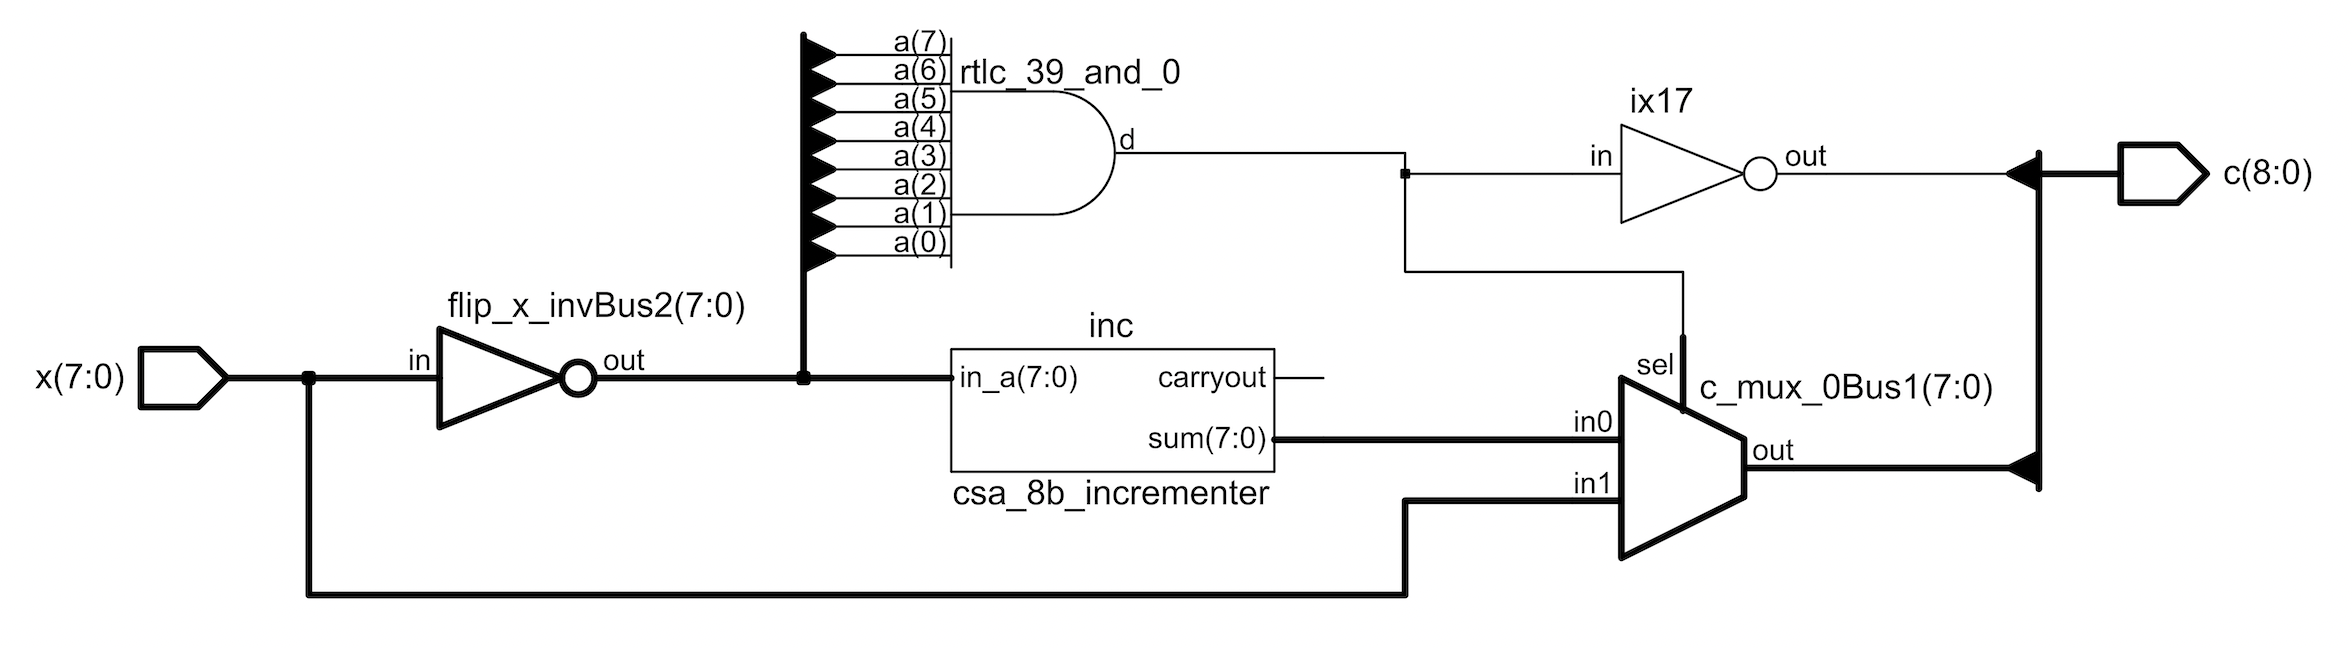
\includegraphics[width=\textwidth]{../img/complementor_rtl.png}
	\label{fig:complementor_rtl}
\end{figure}

\begin{figure}[!ht]
	\centering
	\caption{Simulation Wave Diagram of Complement Generator}
	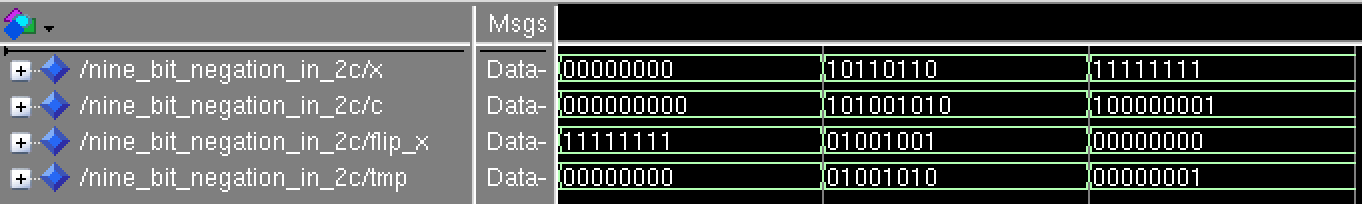
\includegraphics[width=0.9\textwidth]{../img/complementor_sim.png}
	\label{fig:complementor_sim}
\end{figure}

\paragraph{Booth Stage 0}
\figref{fig:booth_stage_0_rtl} and \expref{exp:booth_stage_0} present the hardware implementation and the logic expression of the block.
As the figure suggested, a booth stage block takes the 8-bit operand multiplicand and its 9-bit negation and two of the rightmost bits of the operand multiplier
as input, and composes the 16-bit extended partial product as output by a 4-to-1 mux. The width of the \(extended\_sign\_bits\) will be 6.
The simulation result is shown in \figref{fig:booth_stage_0_sim}.

\begin{figure}[!ht]
	\centering
	\caption{Synthesized RTL Diagram of Booth Stage 0 Block}
	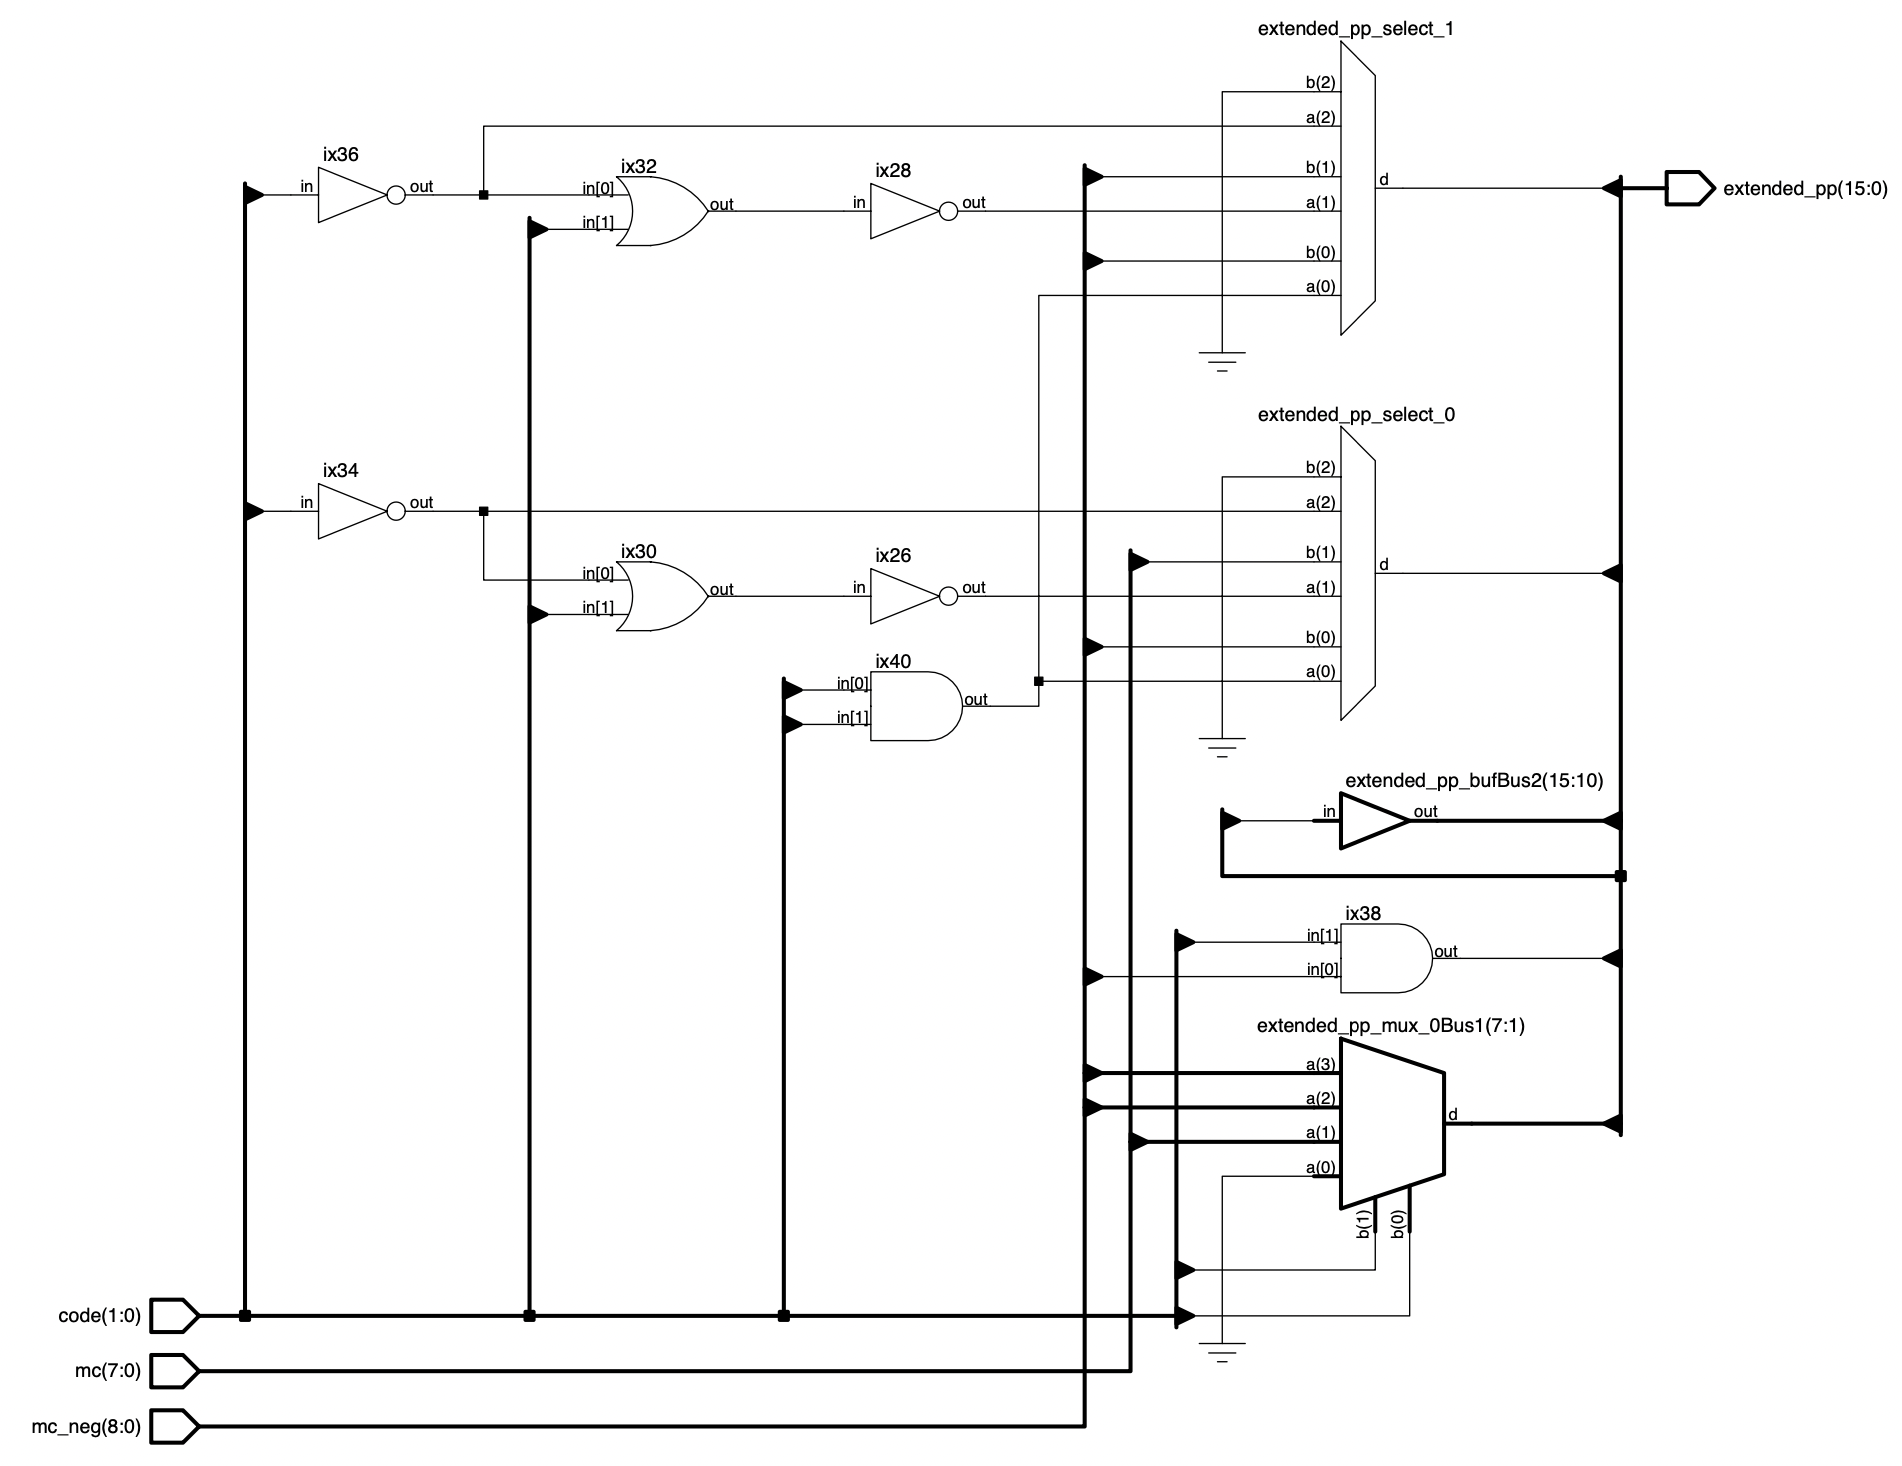
\includegraphics[width=\textwidth]{../img/booth_stage_0_rtl.png}
	\label{fig:booth_stage_0_rtl}
\end{figure}

\clearpage

\begin{equation}
	\begin{array}{c}
		partial\_product =
		\begin{cases}
			0000000000,                 & \text{if } code = 00       \\
			concat(00, mc),             & \text{if } code = 01       \\
			concat(mc\_neg, 0),         & \text{if } code = 10       \\
			concat(mc\_neg(8),mc\_neg), & \text{else } code = others
		\end{cases} \\
		extended\_sign\_bits = (others => partical\_product(9))  \\
		extended\_pp = concat(extended\_sign\_bits, partial\_product)
	\end{array}
	\label{exp:booth_stage_0}
\end{equation}

\begin{figure}[!ht]
	\centering
	\caption{Simulation Wave Diagram of Booth Stage 0 Block}
	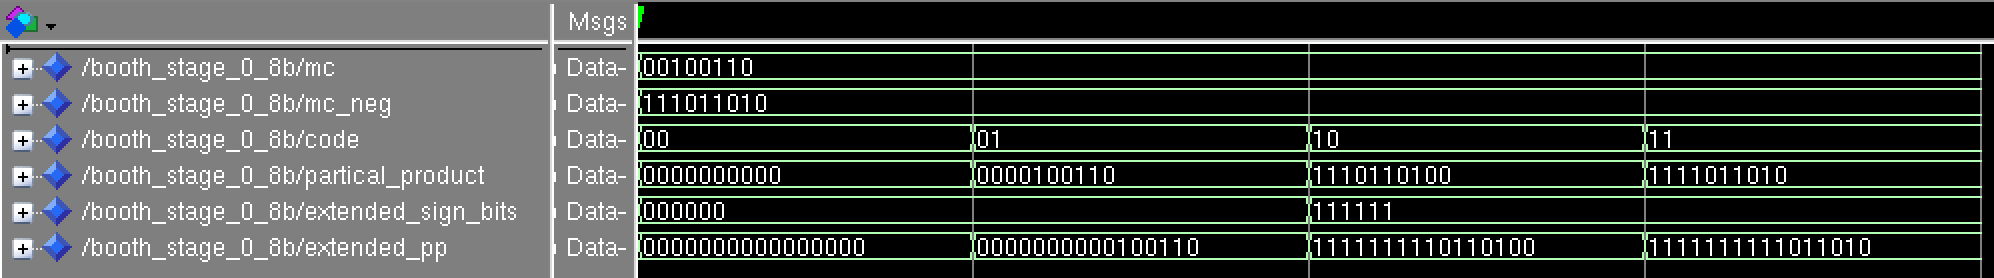
\includegraphics[width=\textwidth]{../img/booth_stage_0_sim.png}
	\figurenote{Four code values were provided to simulate the \(extended\_pp\).}
	\label{fig:booth_stage_0_sim}
\end{figure}

\paragraph{Booth Stage 1}
\figref{fig:booth_stage_1_rtl} and \expref{exp:booth_stage_1} present the hardware implementation and the logic expression of the block.
Different from booth stage 0 block, this stage takes 3 bits from the operand multiplier.
With considering the right shift during the algorithm, the width of the \(extended\_sign\_bits\) will be 4,
and \textquote{00} will be added to the end.
The simulation result is shown in \figref{fig:booth_stage_1_sim}.

\begin{figure}[!ht]
	\centering
	\caption{Synthesized RTL Diagram of Booth Stage 1 Block}
	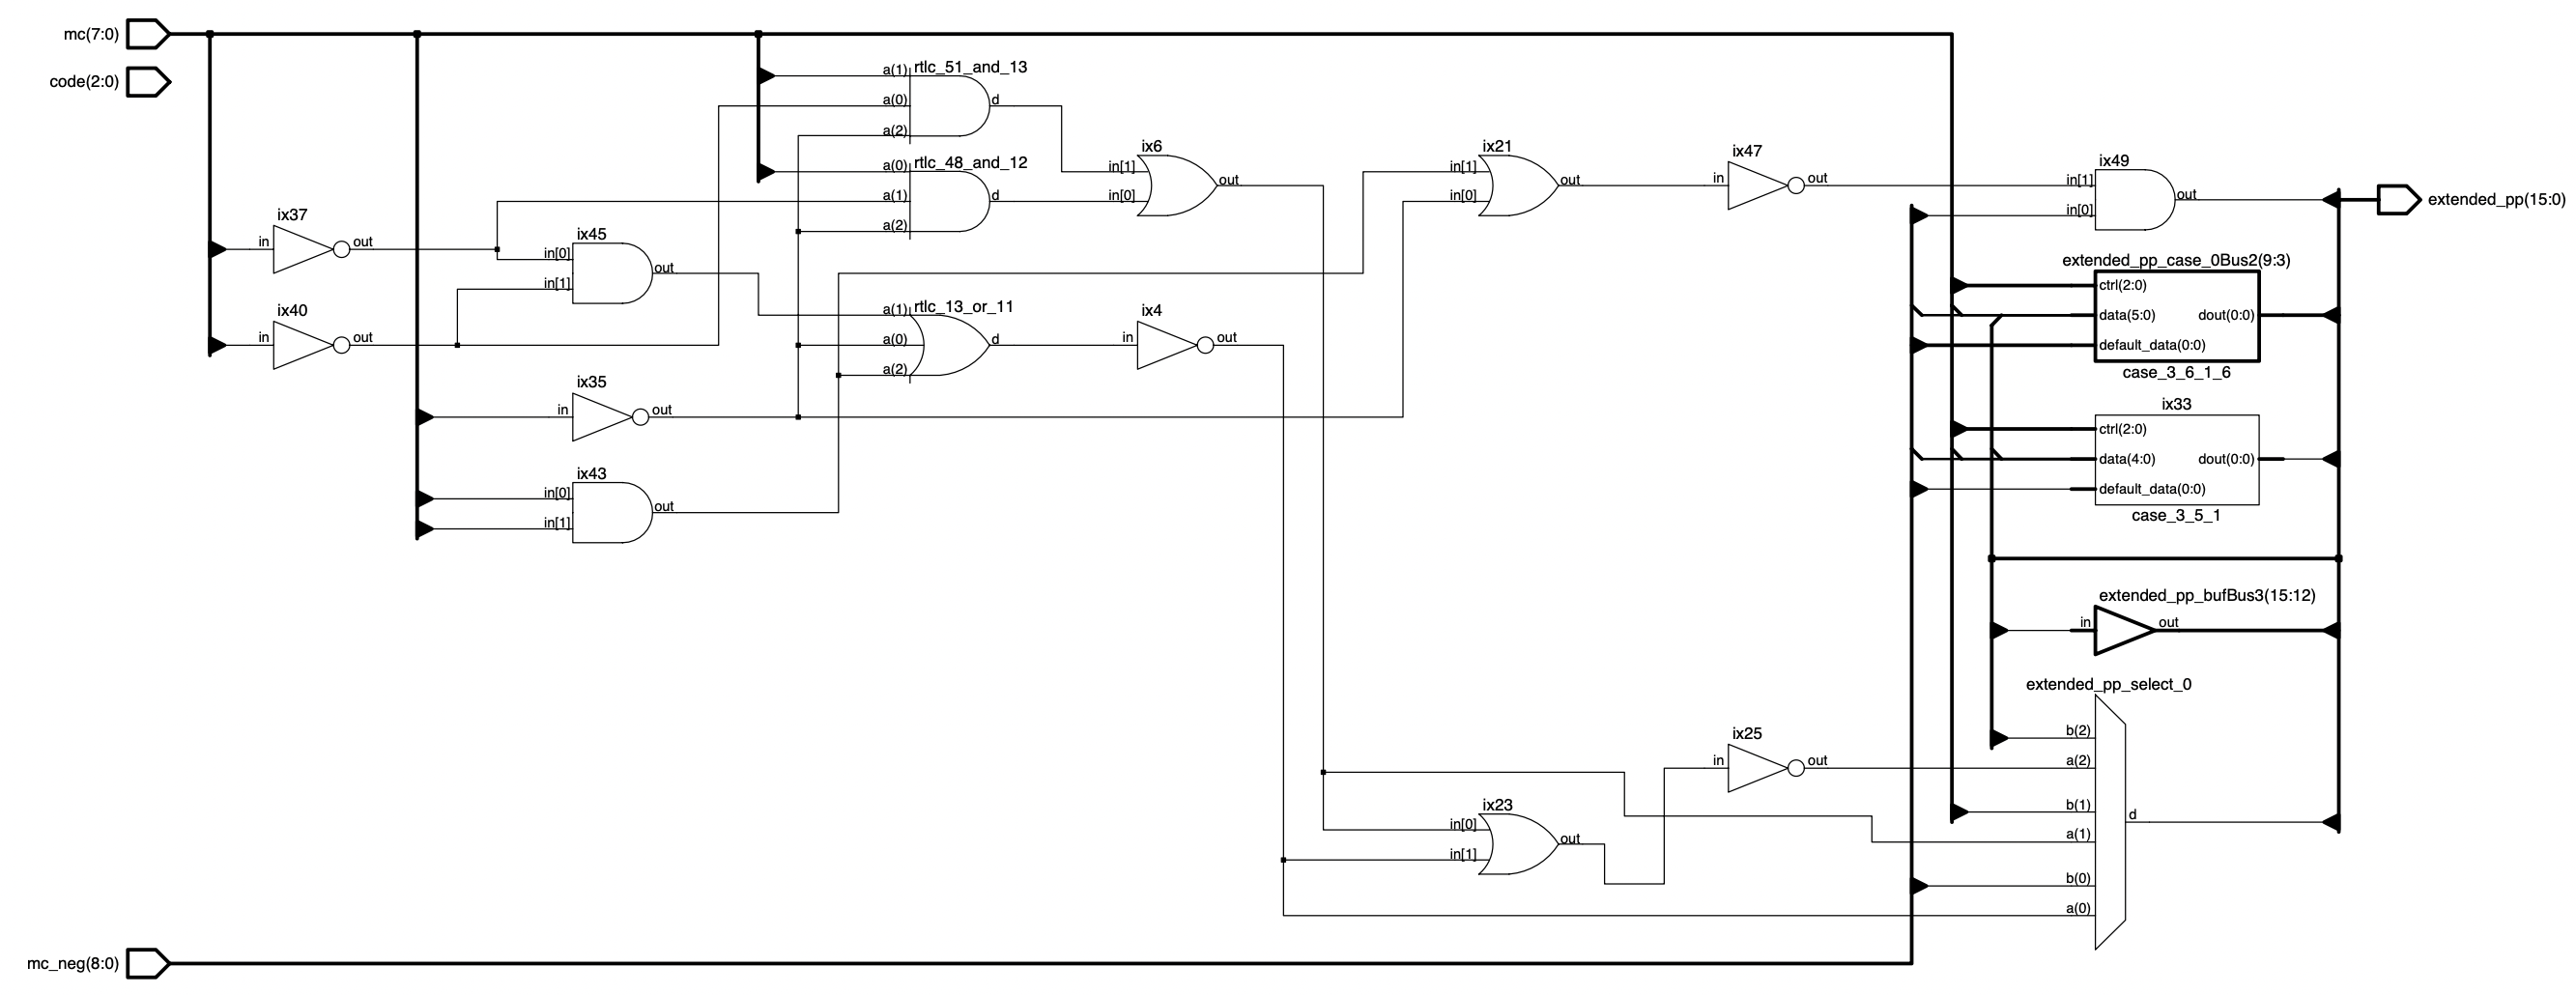
\includegraphics[width=\textwidth]{../img/booth_stage_1_rtl.png}
	\label{fig:booth_stage_1_rtl}
\end{figure}

\begin{equation}
	\begin{array}{c}
		partial\_product =
		\begin{cases}
			0000000000,                 & \text{if } code = 000 | 111 \\
			concat(00, mc),             & \text{if } code = 001 | 010 \\
			concat(0, mc, 0),           & \text{if } code = 011       \\
			concat(mc\_neg, 0),         & \text{if } code = 100       \\
			concat(mc\_neg(8),mc\_neg), & \text{else } code = others
		\end{cases} \\
		extended\_sign\_bits = (others => partical\_product(9))   \\
		extended\_pp = concat(extended\_sign\_bits, partial\_product, 00)
	\end{array}
	\label{exp:booth_stage_1}
\end{equation}

\begin{figure}[!ht]
	\centering
	\caption{Simulation Wave Diagram of Booth Stage 1 Block}

	\subfloat[With Code Values: 000/001/010/011]{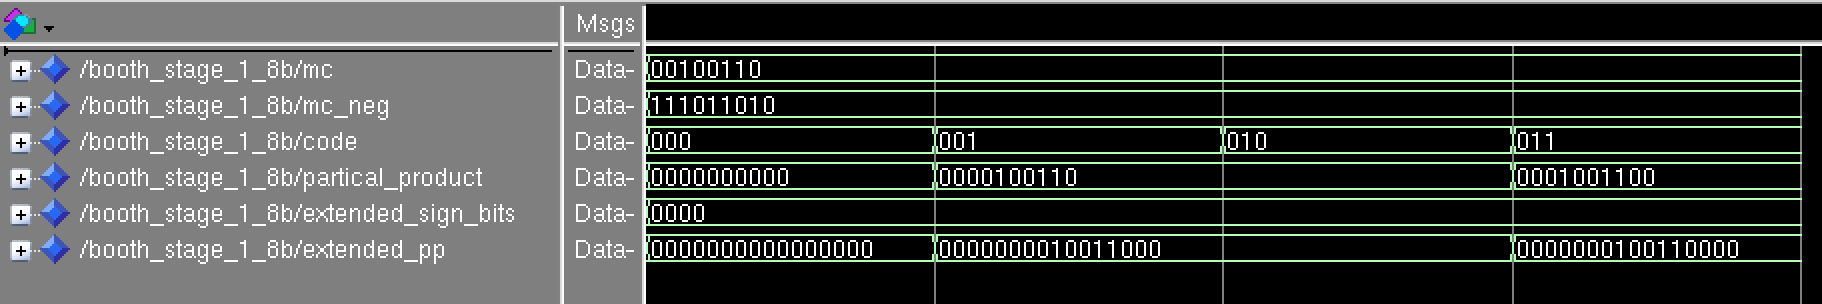
\includegraphics[width=\textwidth]{./img/booth_stage_1_sim_1.png}}
	\hspace{0.5cm}
	\subfloat[With Code Values: 100/101/110/111]{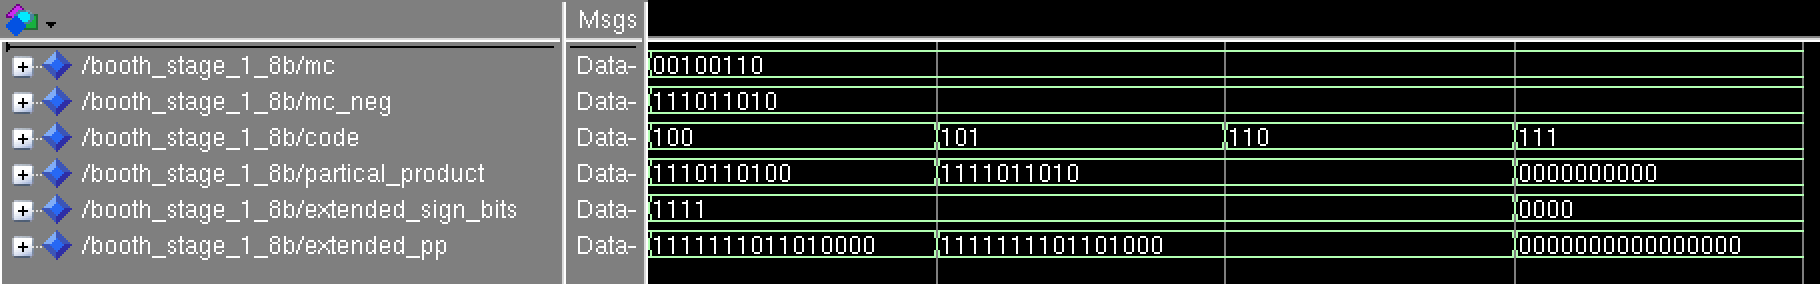
\includegraphics[width=\textwidth]{./img/booth_stage_1_sim_2.png}}

	\figurenote{Eight code values were provided to simulate the \(extended\_pp\).}
	\label{fig:booth_stage_1_sim}
\end{figure}

\paragraph{Booth Stage 2, 3, and 4}
Booth stage 2 and 3 blocks share the same idea of booth stage 1 except they shift more bit to the right.
As for the booth stage 4 block, it only takes the MSB from the operand multiplier. \expref{exp:booth_stage_4} shows its logic.

\begin{equation}
	\begin{array}{c}
		extended\_pp =
		\begin{cases}
			0000000000000000,    & \text{if } code = 0        \\
			concat(mc,00000000), & \text{else } code = others
		\end{cases} \\
	\end{array}
	\label{exp:booth_stage_4}
\end{equation}

\subsection{8-bit Triple Operands Multiplier Circuit Implementation}

Once the 16-bit product of \textbf{\(A^2\)} which is marked as \(product\_aa\) is calculated, it will then multiply with the 8-bit input \(B\).
To perform multiplication with a 16-bit operand and an 8-bit operand, the circuit divides the 16-bit operand into two 8-bit operands.
This is to reuse the 8-bit multiplier block that is designed before.

The product of multiplying the higher 8-bit of \(product\_aa\) and \(B\) will be marked as \(product\_haa\_b\), and it will be extended to 24 bits by shifting 8 bits rightwards.
The product of multiplying the lower 8-bit of \(product\_aa\) and \(B\) will be marked as \(product\_laa\_b\), and it will be extended to 24 bits by adding 8 zeros to its left.
Then adds those two extended 24-bit numbers together will be the result of \textbf{\(A^2 \ast B\)}.

\figref{fig:tri_rtl} presents the RTL description of the circuit and \figref{fig:tri_sim} presents the simulation result.
\expref{exp:tri} shows the arithmetic process of the \textbf{\(A^2 \ast B\)}.

\begin{equation}
	\begin{array}{c}
		aa = a \ast a                     \\
		laa\_b = aa[7, 0] \ast b          \\
		haa\_b = aa[15, 8] \ast b         \\
		aab\_m = concat(haa\_b, 00000000) \\
		aab\_l = concat(00000000, laa\_b) \\
		p = aab\_m + aab\_l
	\end{array}
	\label{exp:tri}
\end{equation}

\begin{figure}[!ht]
	\centering
	\caption{Synthesized RTL Diagram of Triple 8-bit Operands Multiplier Circuit}
	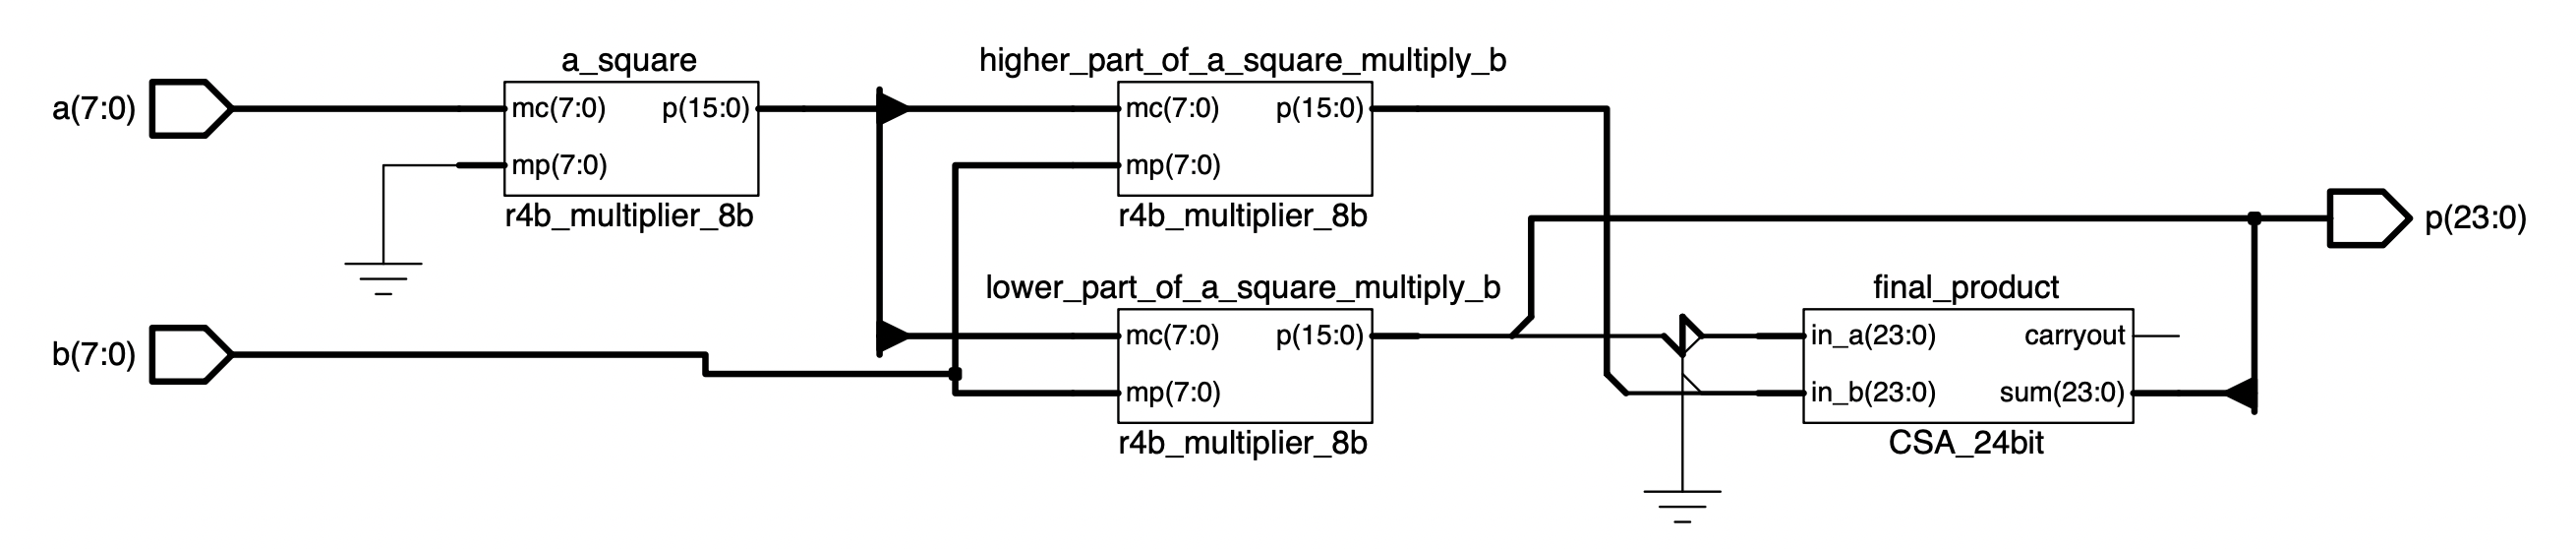
\includegraphics[width=\textwidth]{../img/tri_rtl.png}
	\label{fig:tri_rtl}
\end{figure}

\begin{figure}[!ht]
	\centering
	\caption{Simulation Wave Diagram of Triple 8-bit Operands Multiplier Circuit}
	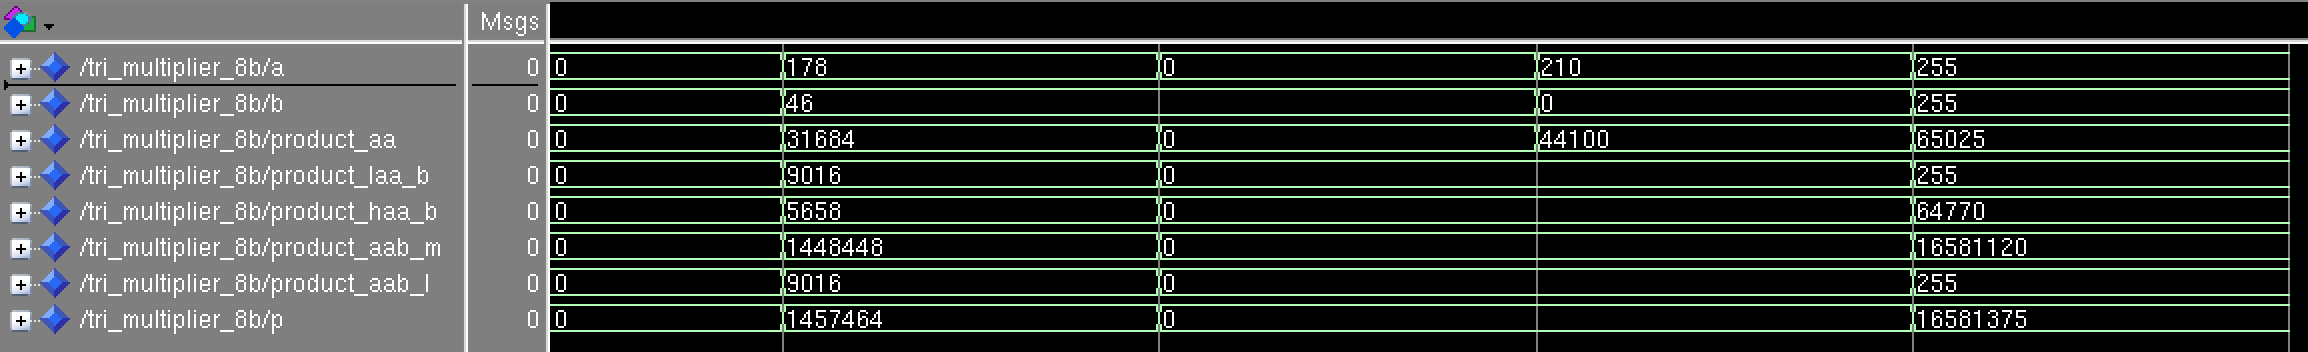
\includegraphics[width=\textwidth]{../img/tri_sim.png}
	\label{fig:tri_sim}
\end{figure}

\newpage
\subsection{16-bit Triple Operands Multiplier Circuit Implementation}

Like the 8-bit version, the 16-bit implementation of the booth multiplier will need 9 blocks of booth stage to calculate 9 partial products
and a 17-bit negation complement generator.
Because of the characteristic of the algorithm, the 16-bit version can not reuse or extend from the 8-bit version circuit designed before.
Hence the circuit will need to build every block from scratch.
\textbf{This is one of the drawbacks of the booth algorithm: lack of expandability.}

\figref{fig:tri_16b_rtl} presents the RTL description of the triple 16-bit operands multiplier circuit
and \figref{fig:tri_16b_sim} presents the simulation result. \figref{fig:overview_booth_16b_rtl} presents the RTL description of the 16-bit booth multiplier circuit.

\begin{figure*}[!ht]
	\centering
	\caption{Synthesized RTL Diagram of 16-bit Radix-4 Booth Multiplier}
	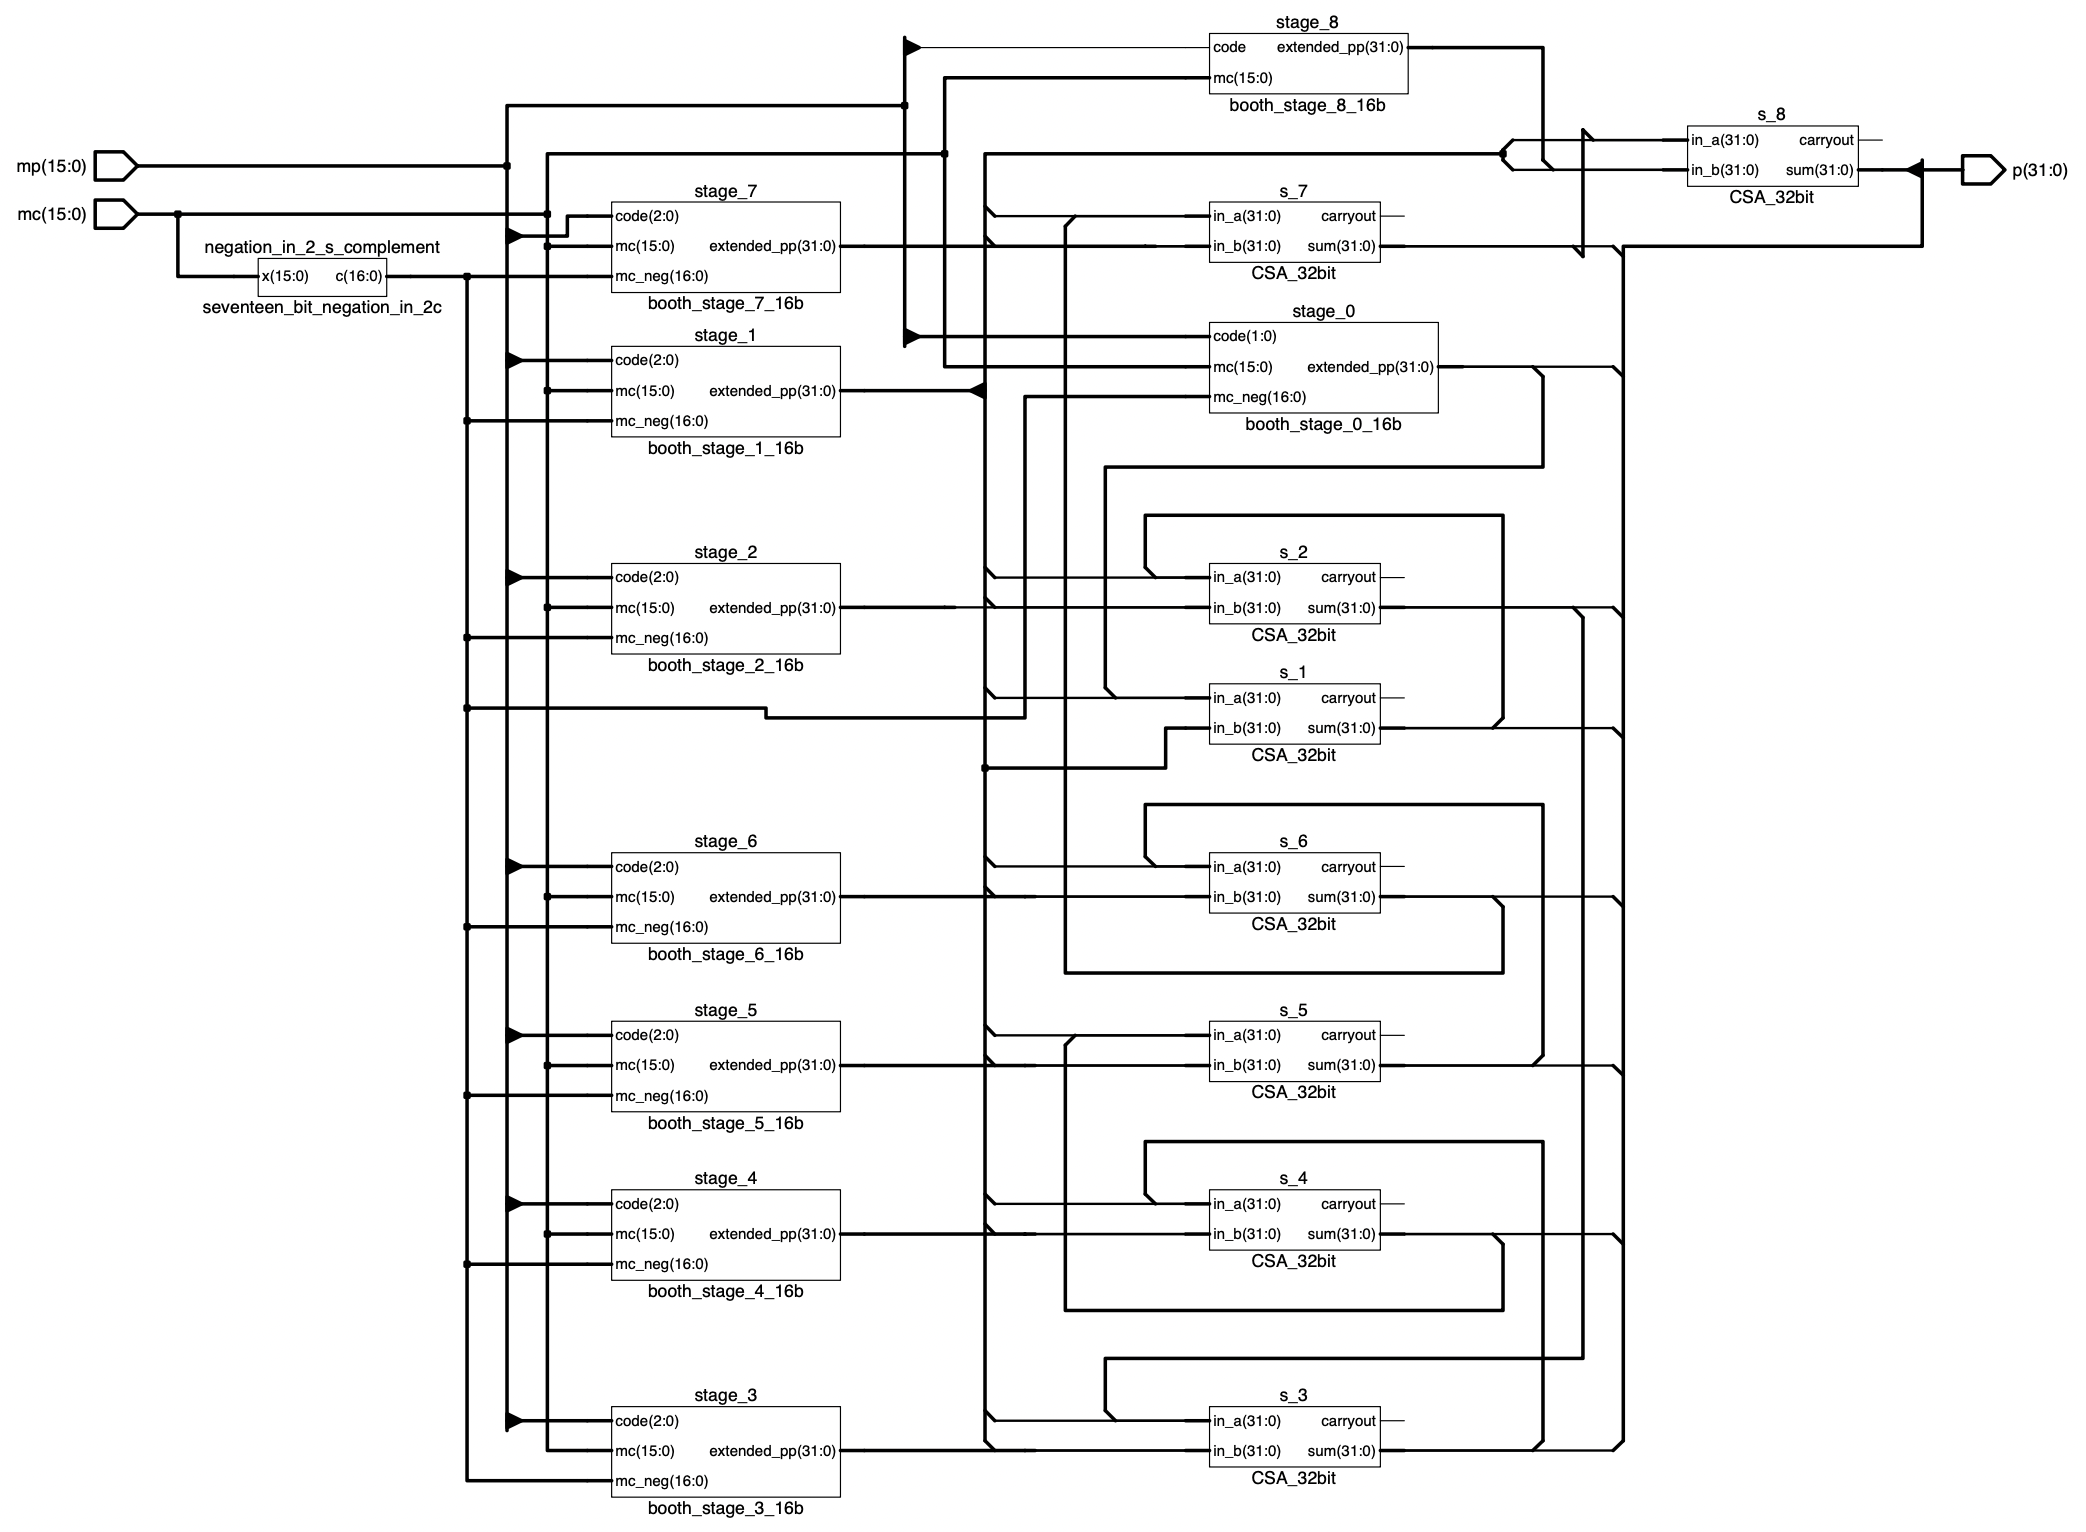
\includegraphics[width=\textwidth]{../img/overview_booth_16b_rtl.png}
	\label{fig:overview_booth_16b_rtl}
\end{figure*}

\begin{figure}[!ht]
	\centering
	\caption{Synthesized RTL Diagram of Triple 16-bit Operands Multiplier Circuit}
	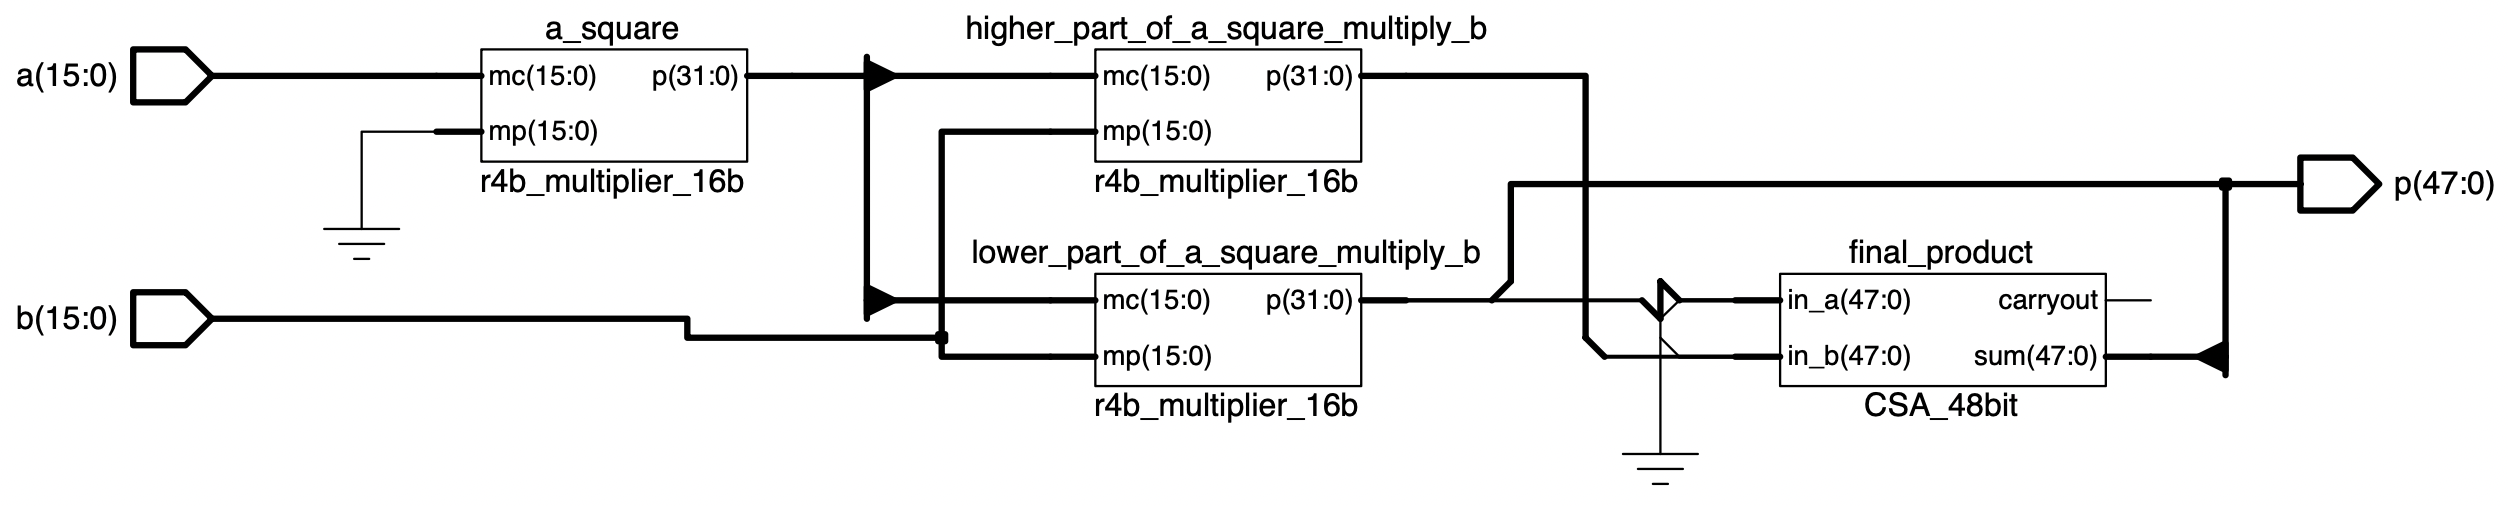
\includegraphics[width=\textwidth]{../img/tri_16b_rtl.png}
	\label{fig:tri_16b_rtl}
\end{figure}

\begin{figure}[!ht]
	\centering
	\caption{Simulation Wave Diagram of Triple 16-bit Operands Multiplier Circuit}
	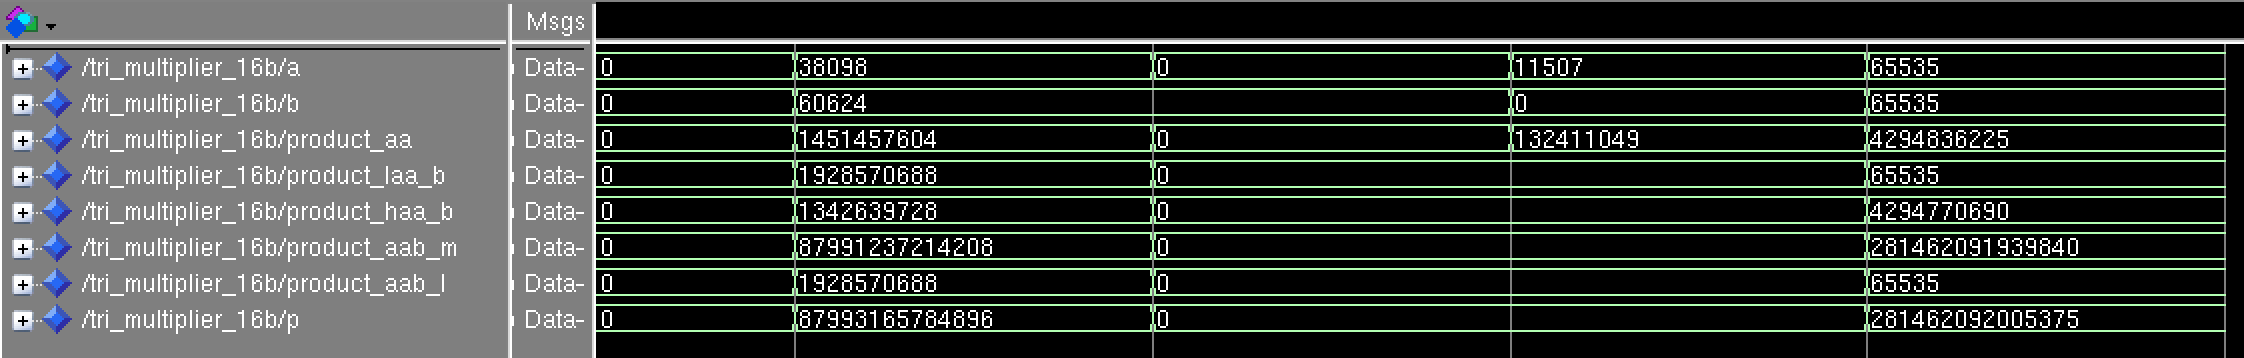
\includegraphics[width=\textwidth]{../img/tri_16b_sim.png}
	\label{fig:tri_16b_sim}
\end{figure}

\clearpage
